\documentclass[tikz,border=6pt]{standalone}
\usepackage{times}
\usepackage{amsmath}
\begin{document}
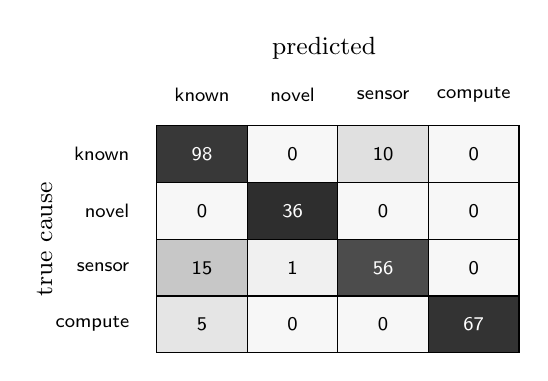
\begin{tikzpicture}[
  font=\sffamily\scriptsize,
  cell/.style={draw, minimum width=1.15cm, minimum height=0.72cm, inner sep=0pt, align=center},
]
\node[font=\small] at (2.7, 4.05) {predicted};
\foreach \j/\lab in {0/known, 1/novel, 2/sensor, 3/compute} {
  \node at ({1.15*\j+1.15}, 3.45) {\lab};
}
\foreach \i/\lab in {0/known, 1/novel, 2/sensor, 3/compute} {
  \node[anchor=east] at (0.35, {2.7-0.72*\i}) {\lab};
}
% known row 98 0 10 0 / 108
\node[cell, fill=black!78, text=white] at (1.15, 2.70) {98};
\node[cell, fill=black!3] at (2.30, 2.70) {0};
\node[cell, fill=black!12] at (3.45, 2.70) {10};
\node[cell, fill=black!3] at (4.60, 2.70) {0};
% novel 0 36 0 0 / 36
\node[cell, fill=black!3] at (1.15, 1.98) {0};
\node[cell, fill=black!82, text=white] at (2.30, 1.98) {36};
\node[cell, fill=black!3] at (3.45, 1.98) {0};
\node[cell, fill=black!3] at (4.60, 1.98) {0};
% sensor 15 1 56 0 / 72
\node[cell, fill=black!22] at (1.15, 1.26) {15};
\node[cell, fill=black!6] at (2.30, 1.26) {1};
\node[cell, fill=black!70, text=white] at (3.45, 1.26) {56};
\node[cell, fill=black!3] at (4.60, 1.26) {0};
% compute 5 0 0 67 / 72
\node[cell, fill=black!10] at (1.15, 0.54) {5};
\node[cell, fill=black!3] at (2.30, 0.54) {0};
\node[cell, fill=black!3] at (3.45, 0.54) {0};
\node[cell, fill=black!80, text=white] at (4.60, 0.54) {67};
\node[rotate=90, font=\small] at (-0.85, 1.62) {true cause};
\end{tikzpicture}
\end{document}
